\chapter{Recherche de résonances de spin 1 -- courbes de limites}

Les courbes de limites obtenues lors de la combinaison entre l'analyse présentée dans le \cref{chap:zprime} et l'analyse semi-leptonique boostée sont visibles sur les \cref{fig_a1_1,fig_a1_2,fig_a1_3}. Une comparaison entre les limites obtenues par les analyses semi-leptoniques et tout-hadronique est présentée sur les \cref{fig:a1_4,fig:a1_5,fig:a1_6}.

\begin{figure}[tb]
    \centering
    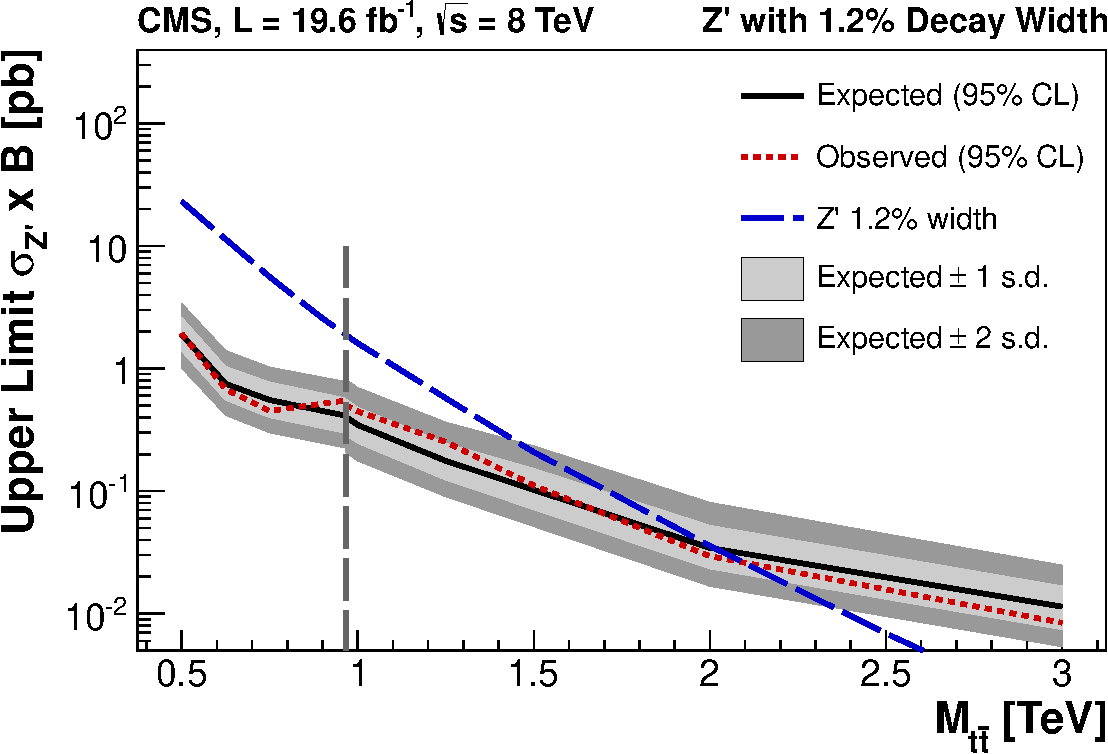
\includegraphics[width=0.8\textwidth]{chapitre7/figs/limits-narrow.pdf}
    \caption{Courbe de limites pour des \zprime, dans l'hypothèse de résonances étroites. La légende est expliquée en détails dans la \cref{fig:limits_narrow_cms_full}.}
    \label{fig_a1_1}
\end{figure}

\begin{figure}[tb]
    \centering
    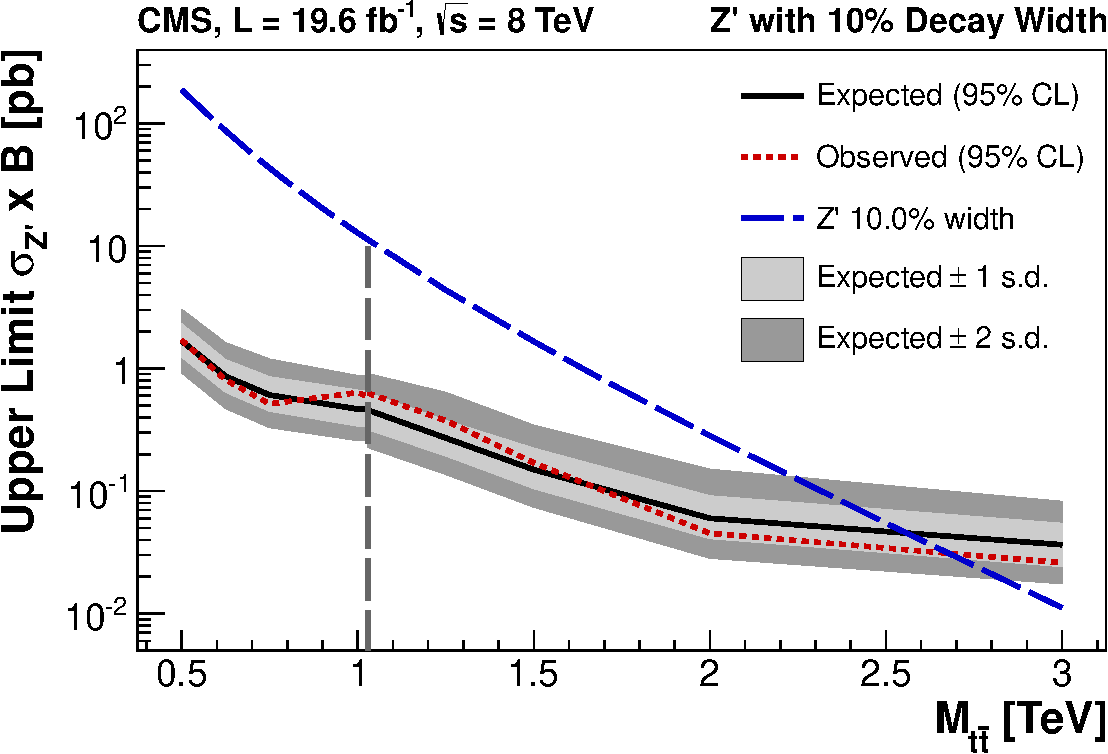
\includegraphics[width=0.8\textwidth]{chapitre7/figs/limits-wide.pdf}
    \caption{Courbe de limites pour des \zprime, dans l'hypothèse de résonances larges. La légende est expliquée en détails dans la \cref{fig:limits_narrow_cms_full}.}
    \label{fig_a1_2}
\end{figure}

\begin{figure}[tb]
    \centering
    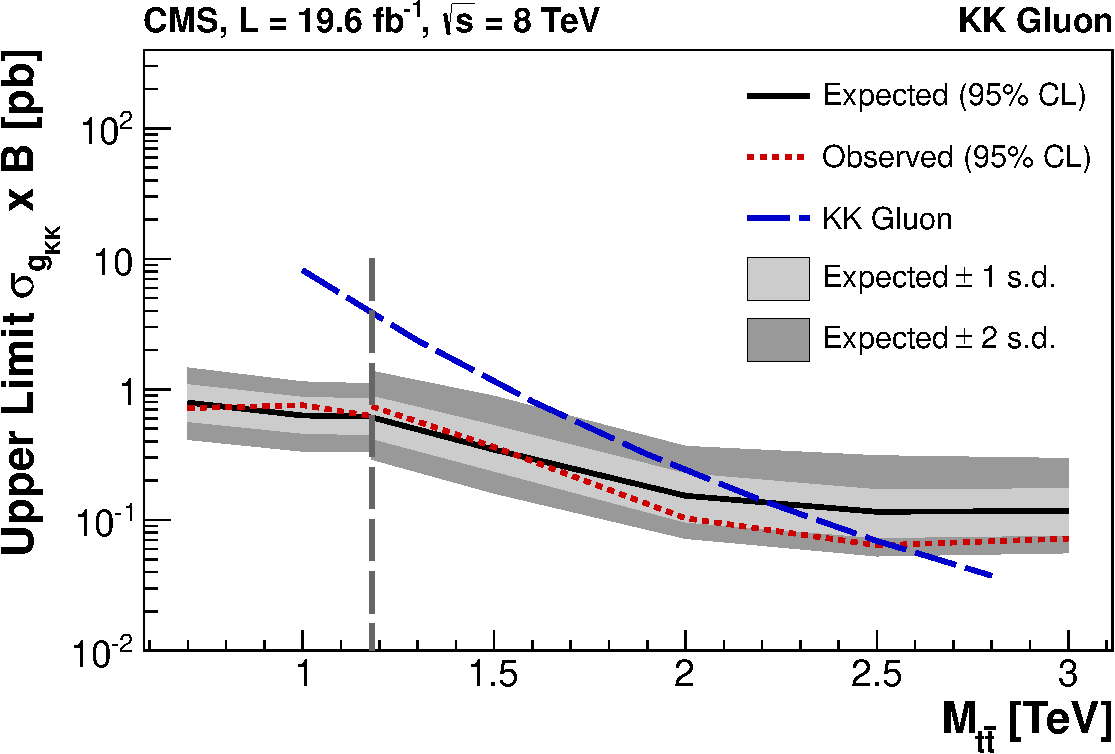
\includegraphics[width=0.8\textwidth]{chapitre7/figs/limits-kk.pdf}
    \caption{Courbe de limites pour des gluons de Kaluza-Klein. La légende est expliquée en détails dans la \cref{fig:limits_narrow_cms_full}.}
    \label{fig_a1_3}
\end{figure}

\begin{figure}[tb]
    \centering
    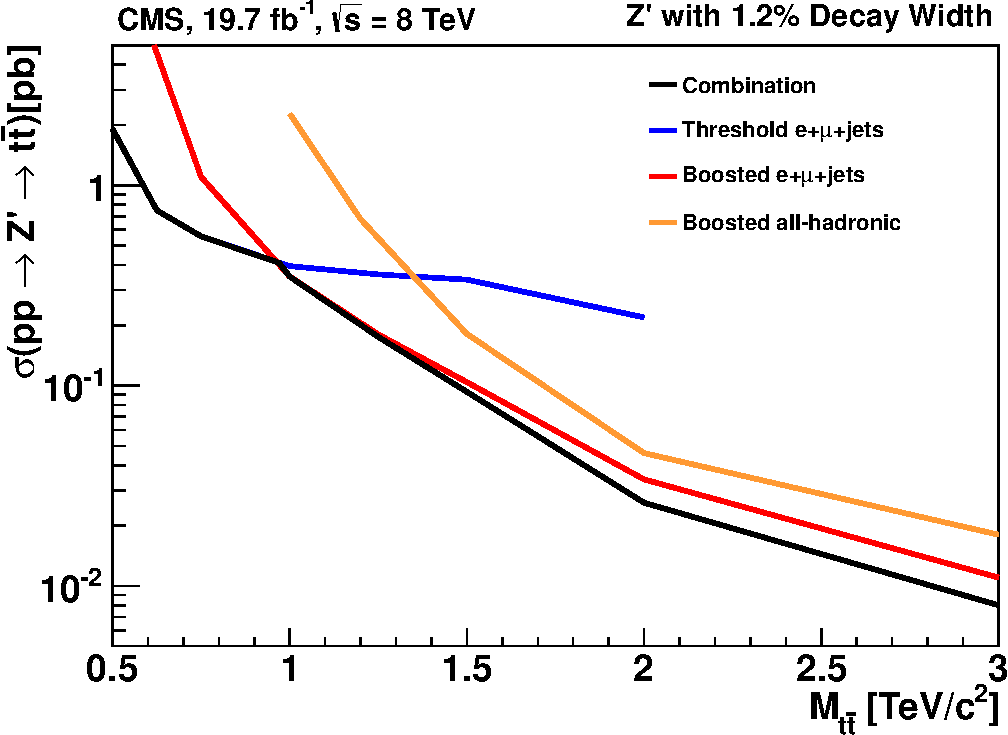
\includegraphics[width=0.8\textwidth]{chapitre7/figs/limit_comparison_narrow_resonances.pdf}
    \caption{Comparaison entre les limites obtenues pour les analyses semi-leptoniques (bleu et rouge) et tout-hadronique (orange) pour un \zprime, dans l'hypothèse de résonances étroites. La combinaison entre ces trois analyses est présentée en noire.}
    \label{fig:a1_4}
\end{figure}

\begin{figure}[tb]
    \centering
    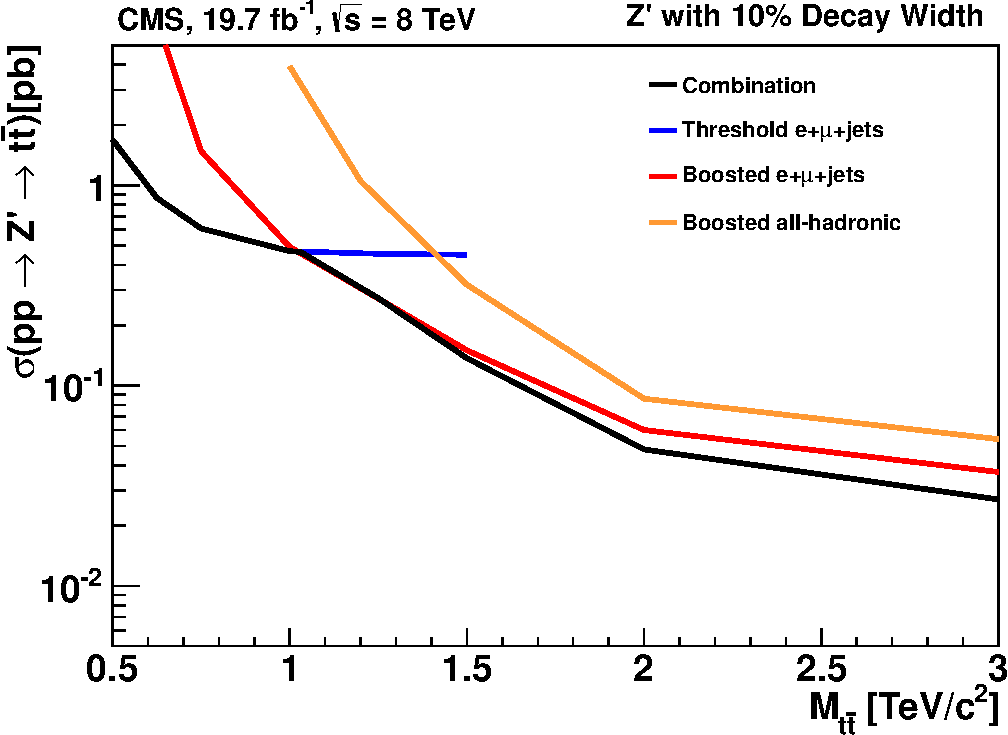
\includegraphics[width=0.8\textwidth]{chapitre7/figs/limit_comparison_wide_resonances.pdf}
    \caption{Comparaison entre les limites obtenues pour les analyses semi-leptoniques (bleu et rouge) et tout-hadronique (orange) pour un \zprime, dans l'hypothèse de résonances larges. La combinaison entre ces trois analyses est présentée en noire.}
    \label{fig:a1_5}
\end{figure}

\begin{figure}[tb]
    \centering
    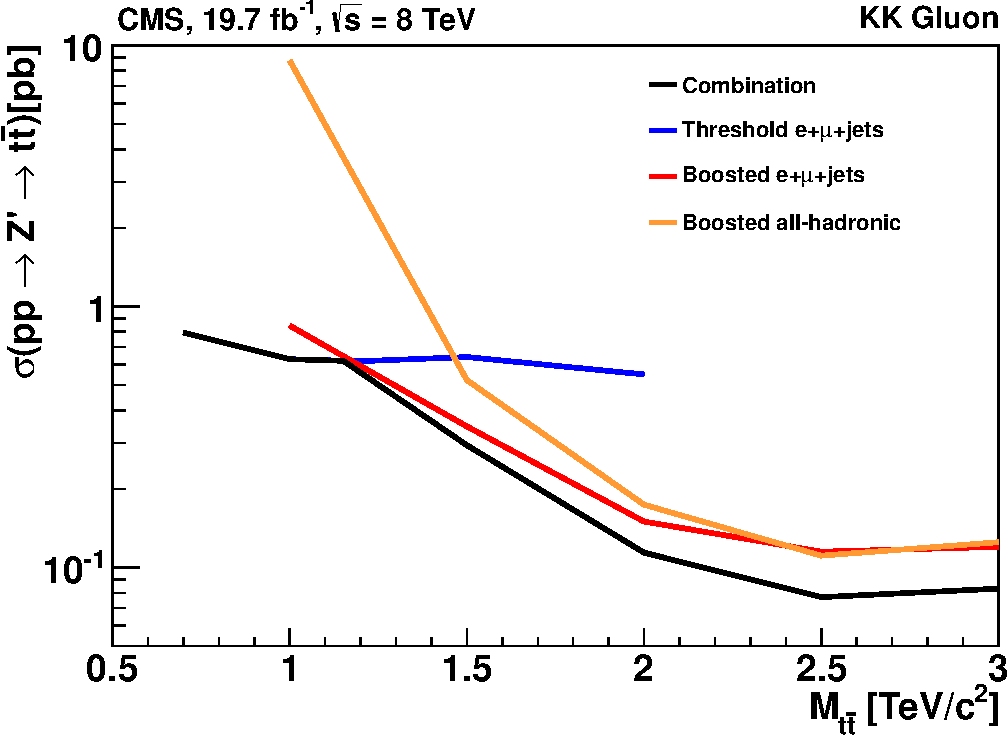
\includegraphics[width=0.8\textwidth]{chapitre7/figs/limit_comparison_rsg_resonances.pdf}
    \caption{Comparaison entre les limites obtenues pour les analyses semi-leptoniques (bleu et rouge) et tout-hadronique (orange) pour un gluon de Kaluza-Klein. La combinaison entre ces trois analyses est présentée en noire.}
    \label{fig:a1_6}
\end{figure}